\subsection{Normalización de datos}
Tomando como ejemplo a los casos especiales para el conjunto de datos utilizado, se puede observar en la Figura \ref{Fig. AgeNorm} que no existen cambio alguno en la distribución de los datos del atributo \emph{age}, mientras que la Figura \ref{Fig. GripNorm} muestra que la elección del método \emph{z-score} para la normalización de datos continuos fue acertada.

\begin{figure}[hb]
	\centering
	\begin{subfigure}{\textwidth}
         \centering
         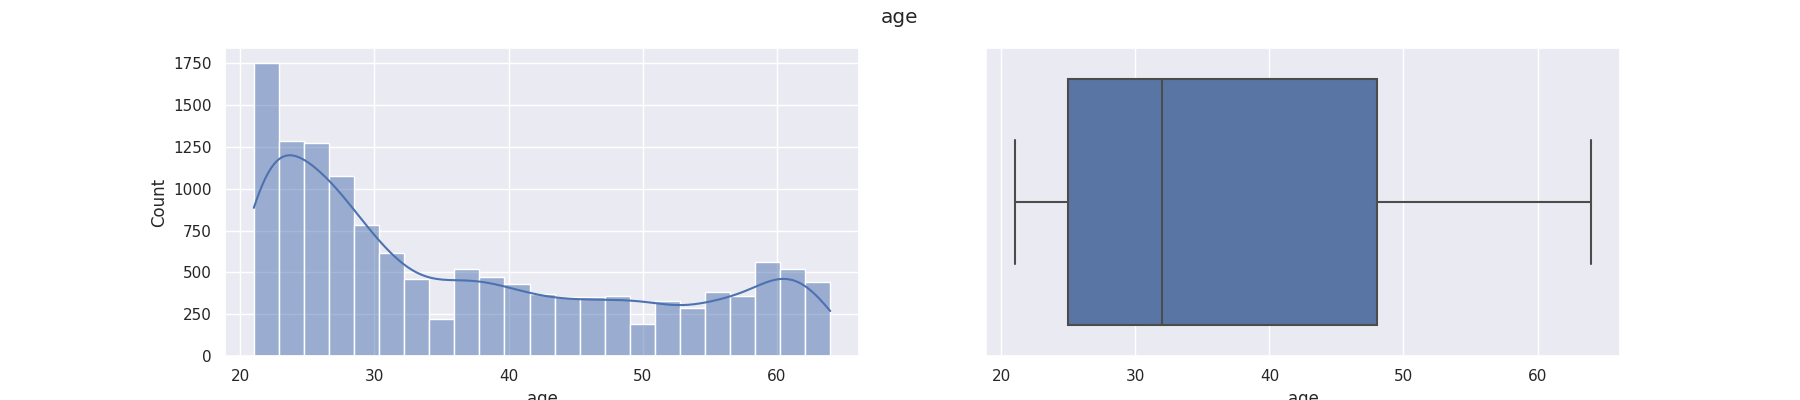
\includegraphics[width=\textwidth]{age_distribution}
         \caption{Distribución previa a normalizar.}
	\end{subfigure}
	\vfill
	\begin{subfigure}{\textwidth}
         \centering
         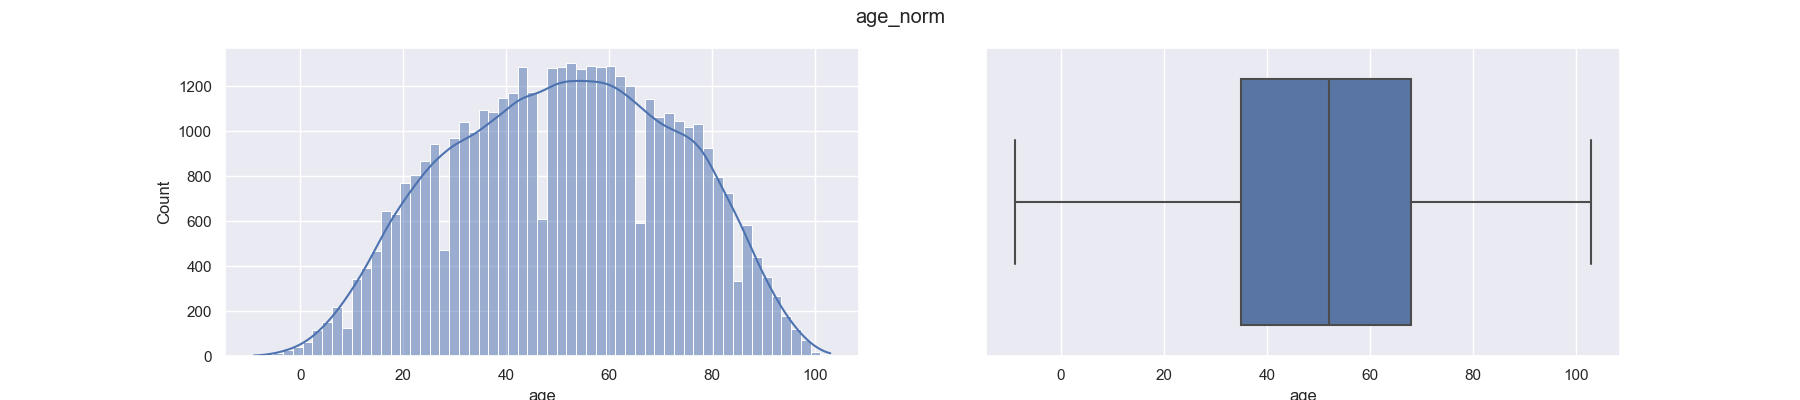
\includegraphics[width=\textwidth]{age_distribution_norm}
         \caption{Distribución posterior a normalizar.}
	\end{subfigure}
	\caption{Distribución de los datos del atributo \emph{age}.}
	\label{Fig. AgeNorm}
\end{figure}

\begin{figure}[ht]
	\centering
	\begin{subfigure}{\textwidth}
         \centering
         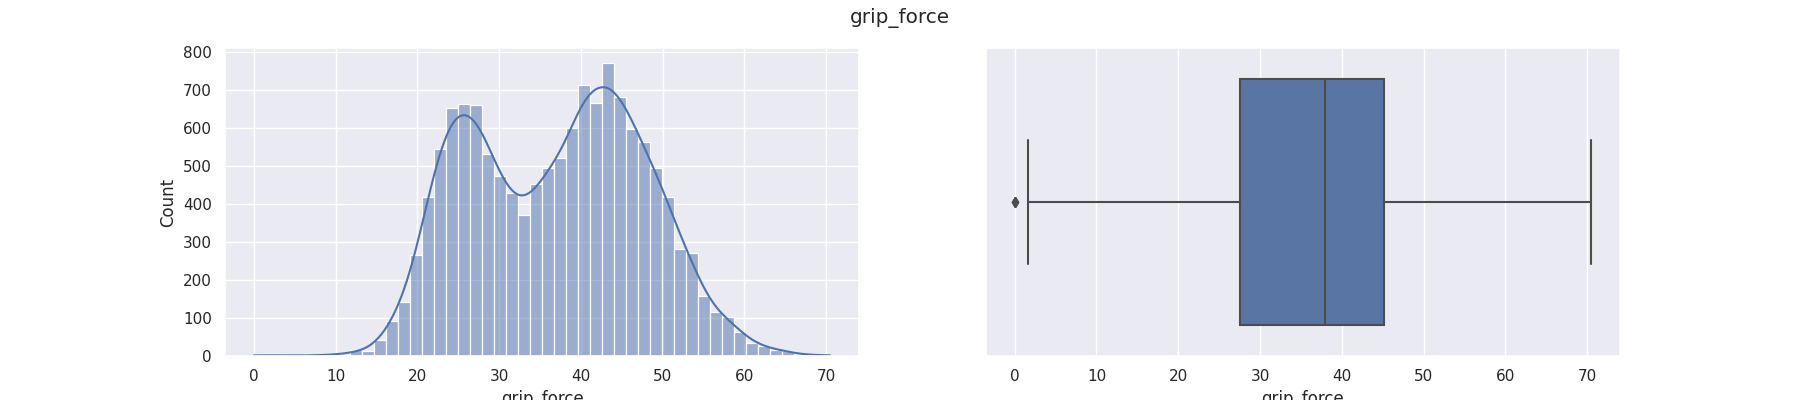
\includegraphics[width=\textwidth]{grip_force_distribution}
         \caption{Distribución previa a normalizar.}
	\end{subfigure}
	\vfill
	\begin{subfigure}{\textwidth}
         \centering
         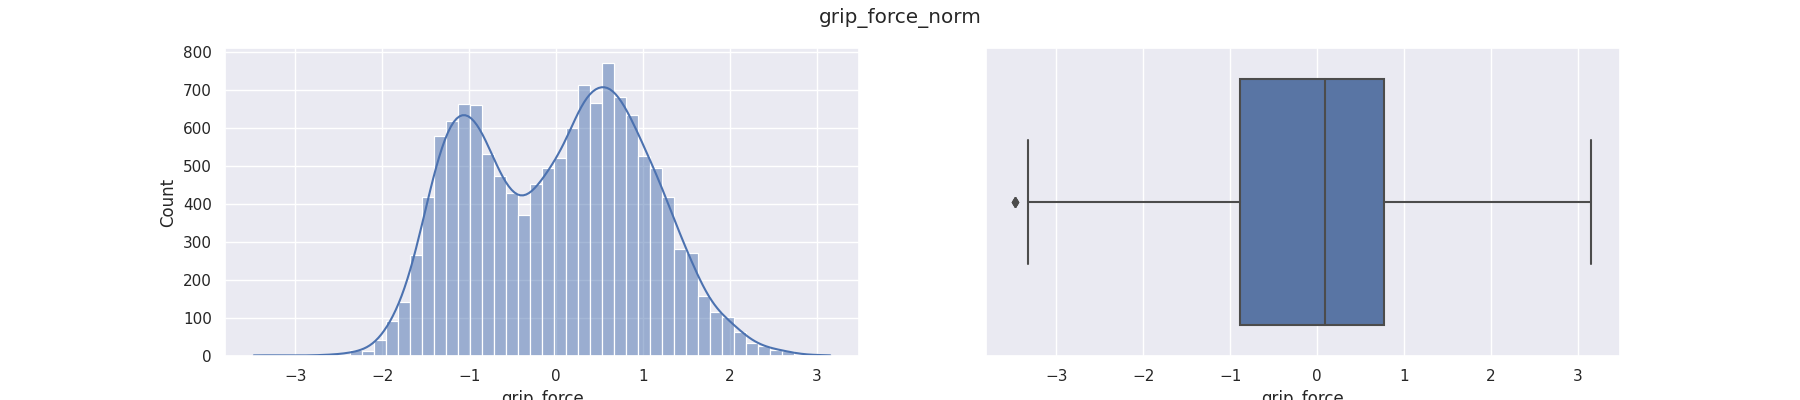
\includegraphics[width=\textwidth]{grip_force_distribution_norm}
         \caption{Distribución posterior a normalizar.}
	\end{subfigure}
	\caption{GripNorm de los datos del atributo \emph{grip\_force}.}
	\label{Fig. AgeNorm}
\end{figure}

\FloatBarrier
\subsection{Análisis de componentes principales}
Relacionado a la extracción de los atributos más relevantes, se logró determinar que dichos atributos fueron \emph{age}, \emph{gender}, \emph{height\_cm} y \emph{weight\_kg}, sumando en conjunuto una ganancia total de $85.36\%$

Para la generación de un subespacio de componentes principales. Se obtuvieron 2 componentes que fueron utilizados de forma satisfactoria en etapas posteriores del desarrollo de este trabajo.

\subsection{Pruebas simples de métodos de clustering}
Observando la distribución real de los clusters del conjunto de datos utilizado (Figura \ref{Fig. TrueClue}), se puede determinar de forma visual que no existe un patrón claro en la distribución de los clusters, lo cual se debería tomar en cuenta al analizar los resultados de los demás métodos de clustering.

El método \emph{K-means} (Figura: \ref{Fig. KMeans} logró obtener los 4 clusters solicitados, sin embargo, se notan discrepancias en la distribución real de los clusters y la propuesta por dicho algoritmo.

Por otro lado, el método \emph{affinity propagation} (Figura: \ref{Fig. AffP} mostró una alerta en su proceso de entrenamiento, donde se indica que los datos no están convergiendo, lo cual ocasiona que el algoritmo termine con poco más de $850$ clusters en su totalidad.

\begin{figure}[ht]
	\centering
	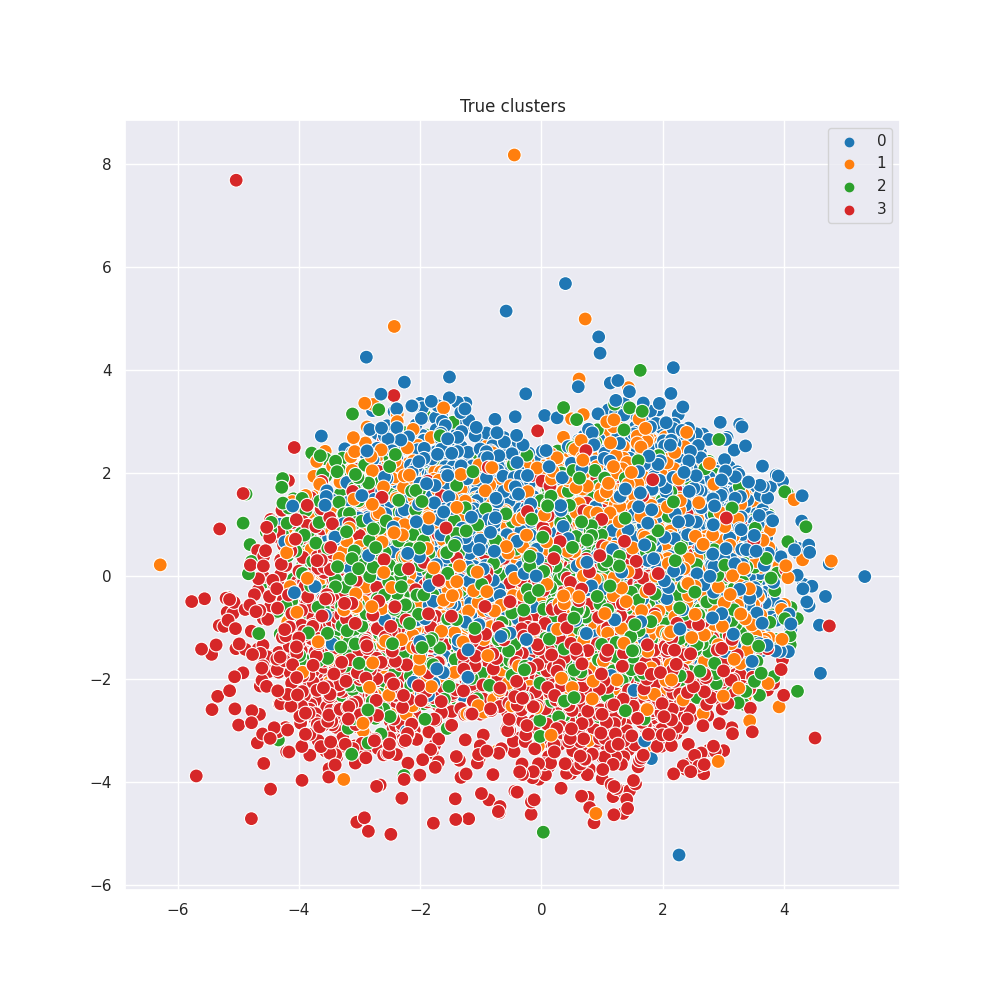
\includegraphics[width=\textwidth]{true_clusters}
	\caption{Distribución real de los clusters existentes en el conjunto de datos.}
	\label{Fig. TrueClue}
\end{figure}

\begin{figure}[ht]
	\centering
	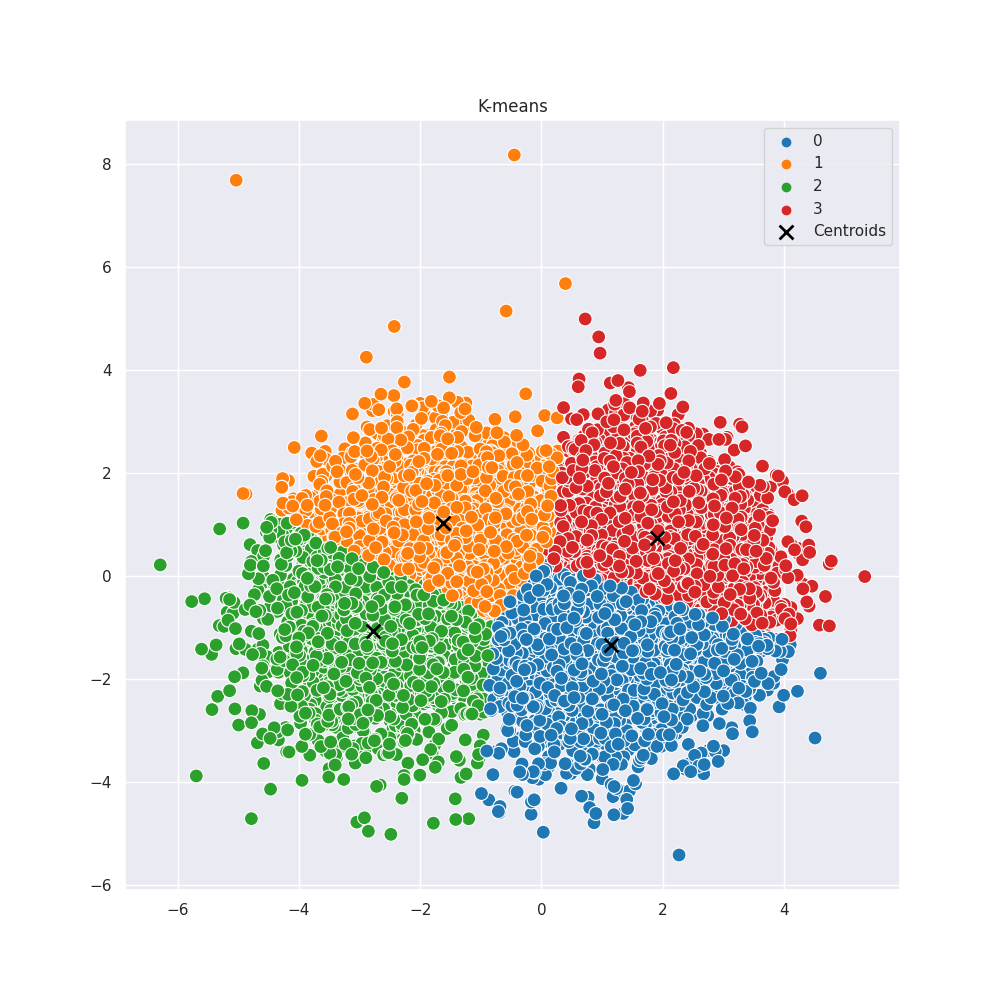
\includegraphics[width=\textwidth]{k_means}
	\caption{Distribución de los clusters propuestos por el algoritmo K-Means.}
	\label{Fig. KMeans}
\end{figure}

\begin{figure}[ht]
	\centering
	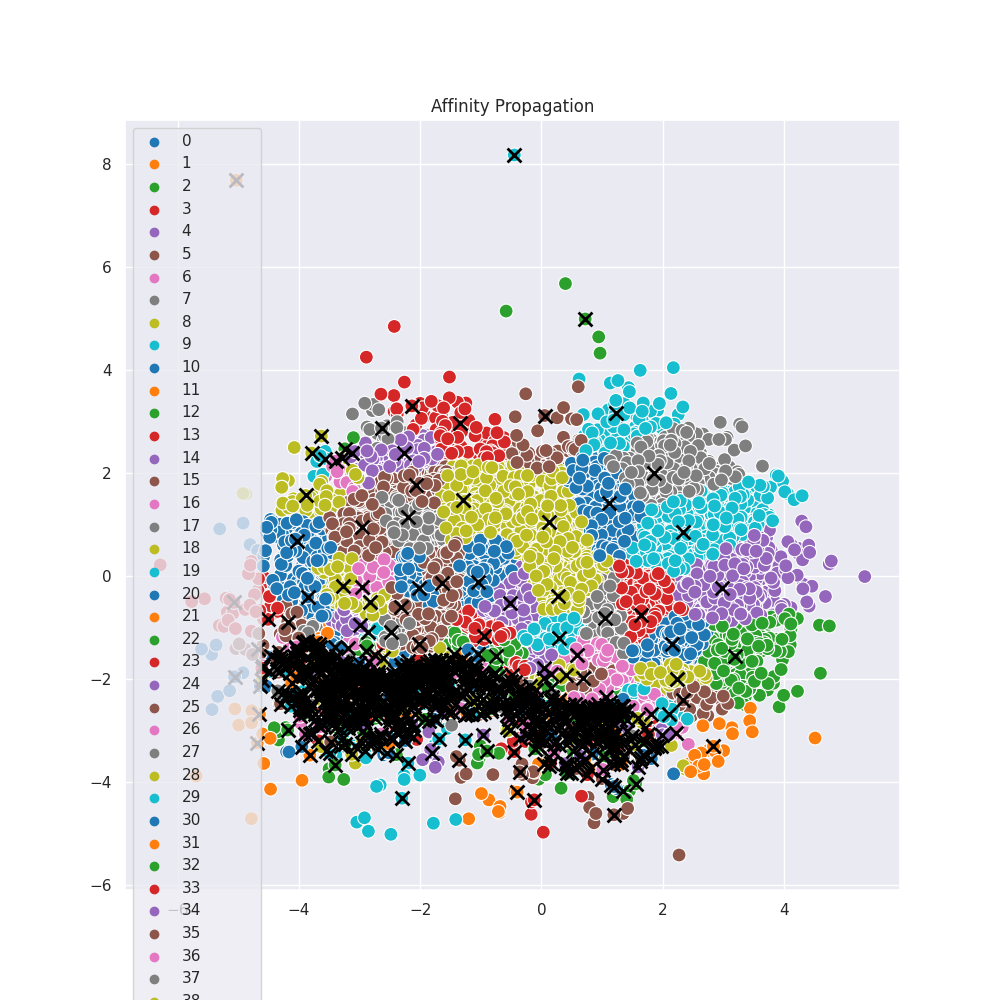
\includegraphics[width=\textwidth]{affinity}
	\caption{Distribución de los clusters propuestos por el algoritmo affinity.}
	\label{Fig. AffP}
\end{figure}

\FloatBarrier
\subsection{Evaluación final de métodos de clustering}
Debido a las grandes diferencias entre la cantidad de clusters determinada por el algoritmo \emph{Affinity}, se optó por solamente evaluar el algoritmo \emph{K-means} mendiante las pruebas de validación cruzada. Tomando un total de 10 repeticiones de entrenamiento se obtuvieron los resultados mostrados en la Figura \ref{Fig. KFold}.

\begin{figure}[ht]
	\centering
	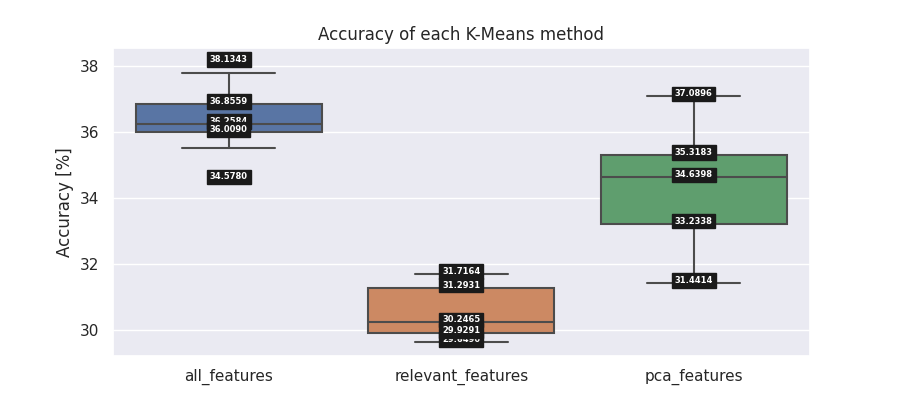
\includegraphics[width=\textwidth]{k_means_accuracies}
	\caption{Exactitud resultante de la validación cruzada aplicada al método K-Means usando diferentes atributos.}
	\label{Fig. KFold}
\end{figure}

